\documentclass[11pt,spanish]{article}

\input{preamble.tex}
\newcommand{\tnum}{1} % reemplace 1 por el número de la tarea
\newcommand{\sem}{2026-2} % reemplace 2024-2 por el semestre correspondiente
\newcommand{\campus}{San joaquin} % reemplace Casa Central por el campus correspondiente
\newcommand{\rolusm}{202473057-6} % reemplace 2025073100-1 por su rol
\newcommand{\namestudent}{Cristobal Duarte} % reemplace Al Goritmo Pérez por su nombre
\newcommand{\deadline}{8 de Septiembre de 2026} % reemplace POR DEFINIR por la fecha de entrega

\headheight=14pt
\linespread{1.3}
\author{\namestudent}
\pagestyle{fancy}
\fancyhf{}
\fancyfoot[R]{\namestudent \\ \rolusm}
\fancyfoot[L]{Campus \campus}
\fancyfoot[C]{\thepage}
\rhead{\sem}
\lhead{INF-221}
\renewcommand{\headrulewidth}{0.4pt}
\renewcommand{\footrulewidth}{0.4pt}
\newbool{programs}
\boolfalse{programs}
\chead{REPORTE TAREA \tnum~}

\title{
  \huge
  \textbf{REPORTE TAREA \tnum~ \\ ALGORITMOS Y COMPLEJIDAD} \\[1ex]
  \emph{\textquote{Más allá de la notación asintótica: Análisis experimental de algoritmos de ordenamiento y multiplicación de matrices.}}
}

\date{
  \small
  \today\\
}

\begin{document}
\maketitle
\thispagestyle{fancy}
\vspace{-1.0\baselineskip}

% Resumen / Abstract
Este trabajo presenta un análisis experimental y comparativo del rendimiento práctico frente a las cotas asintóticas teóricas de cuatro algoritmos de ordenamiento (\textit{MergeSort}, \textit{QuickSort} con partición de Hoare, \textit{PatienceSort} y \texttt{std::sort}) y dos enfoques de multiplicación matricial cuadrada (el método iterativo tradicional \textit{Naive} $\Theta(n^3)$ y el algoritmo \textit{Divide y Vencerás} de Strassen $\mathcal{O}(n^{2.81})$). Se evalúan tiempos de ejecución en CPU de alta precisión y consumos máximos de memoria RAM bajo diversas dimensiones ($N$), topologías de datos y dominios. Los resultados evidencian que en ordenamiento las implementaciones se ajustan estrechamente a $\mathcal{O}(n \log n)$, destacando la baja constante oculta de \texttt{std::sort}. En contraste, en multiplicación matricial la elevada constante oculta y la dispersión en memoria de Strassen provocan que el método \textit{Naive} resulte significativamente superior para todas las instancias evaluadas ($N \le 256$), demostrando el impacto determinante de la jerarquía de memoria física por sobre la complejidad asintótica en rangos prácticos.

% Índice general de contenidos
\tableofcontents
\newpage

\section{Introducción}
El análisis teórico de algoritmos se fundamenta en la caracterización asintótica del costo temporal y espacial mediante las notaciones $\mathcal{O}$, $\Omega$ y $\Theta$ . Estas cotas permiten clasificar funciones según su tasa de crecimiento cuando el tamaño de la entrada $n$ tiende a infinito, abstrayendo deliberadamente factores constantes multiplicativos y términos de orden inferior.

Si bien este modelo proporciona garantías formales independientes de la plataforma de cómputo, en entornos de ejecución reales —gobernados por el modelo abstracto \textit{word-RAM} y arquitecturas físicas contemporáneas— factores como la jerarquía de memoria caché (niveles L1, L2 y L3), la predicción de saltos a nivel de procesador, las asignaciones dinámicas en memoria secundaria y el costo del marco de llamadas recursivas inciden drásticamente en el rendimiento observable. Como consecuencia directa, un algoritmo con una cota asintótica superior puede resultar significativamente más lento que uno de mayor orden de complejidad para rangos prácticos del problema si sus constantes ocultas o su dispersión espacial en memoria son elevadas .

El presente reporte tiene como objetivo confrontar el comportamiento teórico con el desempeño experimental de dos problemas fundamentales:
\begin{enumerate}
    \item \textbf{Ordenamiento de arreglos unidimensionales de enteros:} Estudio comparativo de MergeSort , QuickSort con pivote aleatorio y partición de Hoare , PatienceSort y el algoritmo introspectivo \texttt{std::sort} .
    \item \textbf{Multiplicación de matrices cuadradas de enteros:} Comparación entre el enfoque tradicional iterativo Naive ($\Theta(n^3)$)  y el método Divide y Vencerás de Strassen ($\mathcal{O}(n^{\log_2 7}) \approx \mathcal{O}(n^{2.81})$) .
\end{enumerate}

A través de mediciones empíricas de tiempo de CPU de alta resolución y consumo de memoria máxima residente (RAM), se analiza la incidencia de la estructura previa de los datos, el dominio numérico y el tamaño de la instancia, determinando los límites prácticos y la validez experimental de las cotas asintóticas.


\section{Entorno experimental}
Las pruebas experimentales se ejecutaron en un entorno controlado bajo el sistema operativo macOS (arquitectura ARM64 / Apple Silicon). La compilación de los módulos en C++ se realizó utilizando el compilador nativo \texttt{clang++} (Apple LLVM versión 15+) bajo el estándar \texttt{C++17} y la bandera de optimización \texttt{-O2}.

El protocolo de medición experimental se estructuró de la siguiente forma:
\begin{itemize}
    \item \textbf{Medición Temporal:} Se utilizó el reloj monotónico de alta resolución \texttt{std::chrono::high\_resolution\_clock} provisto por la biblioteca estándar de C++, cronometrando de manera estricta el tiempo de cómputo del algoritmo y aislando por completo las operaciones de entrada/salida (lectura y escritura en disco).
    \item \textbf{Medición Espacial:} El consumo de memoria máxima residente (RAM) se obtuvo mediante la llamada del sistema \texttt{getrusage(RUSAGE\_SELF, ...)}, normalizando el campo \texttt{ru\_maxrss} a kilobytes (KB).
    \item \textbf{Muestreo Estadístico:} Con el fin de mitigar la varianza inducida por procesos concurrentes del sistema operativo, cada configuración experimental se ejecutó sobre tres muestras independientes ($M = \{a, b, c\}$), computando la media aritmética en los análisis posteriores.
\end{itemize}

\section{Resultados y Análisis}
A continuación se presentan y discuten los resultados obtenidos tras ejecutar la batería experimental para el ordenamiento de arreglos y la multiplicación matricial. Se seleccionaron las configuraciones más representativas para contrastar empíricamente el comportamiento asintótico con la realidad del hardware.

\subsection{Ordenamiento de Arreglos Unidimensionales}

Para el problema de ordenamiento se evaluaron los cuatro algoritmos sobre arreglos de tamaño $N \in \{10^1, 10^3, 10^5, 10^7\}$ bajo diversas ordenaciones y dominios numéricos. En la Figura~\ref{fig:sorting_aleatorio} y Figura~\ref{fig:sorting_ascendente} se ilustran los desempeños para entradas aleatorias y ordenadas ascendentemente.

\begin{figure}[htbp]
    \centering
    \begin{minipage}{0.48\textwidth}
        \centering
        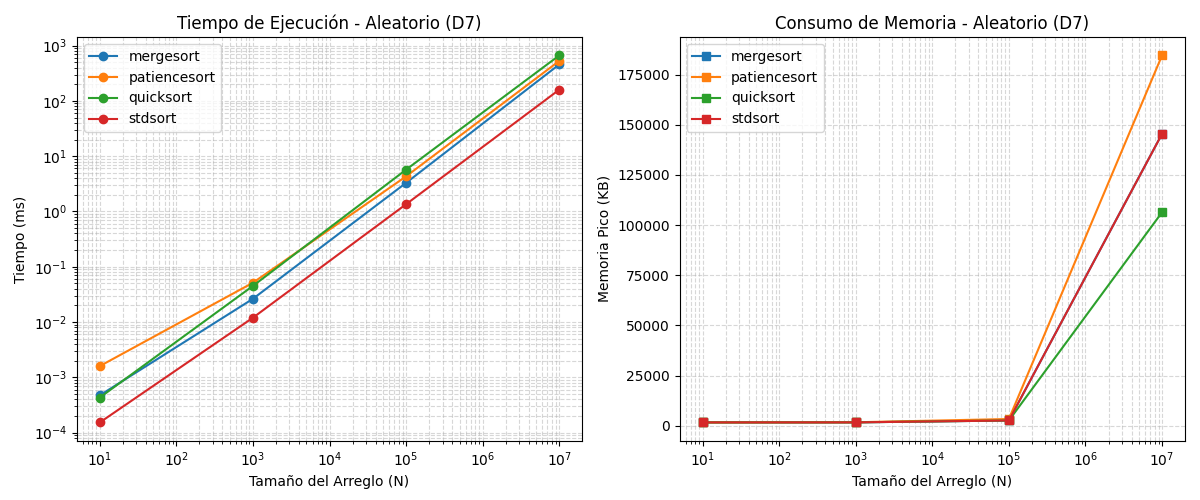
\includegraphics[width=\linewidth]{plots/sorting_aleatorio_D7.png}
        \caption{Tiempo y memoria en arreglos aleatorios ($D7$).}
        \label{fig:sorting_aleatorio}
    \end{minipage}\hfill
    \begin{minipage}{0.48\textwidth}
        \centering
        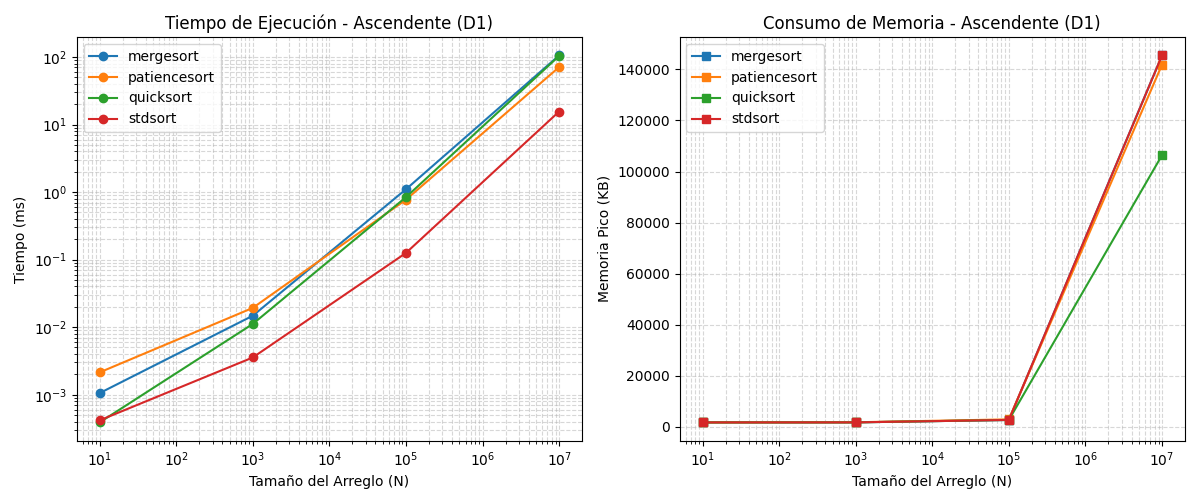
\includegraphics[width=\linewidth]{plots/sorting_ascendente_D1.png}
        \caption{Tiempo y memoria en arreglos ordenados ($D1$).}
        \label{fig:sorting_ascendente}
    \end{minipage}
\end{figure}

\begin{table}[htbp]
\centering
\small
\caption{Tiempo de ejecución promedio (ms) y memoria pico (KB) para $N = 10^7$.}
\label{tab:sorting_summary}
\begin{tabular}{llrrrr}
\toprule
\textbf{Distribución} & \textbf{Métrica} & \textbf{MergeSort} & \textbf{QuickSort} & \textbf{PatienceSort} & \textbf{std::sort} \\
\midrule
Aleatorio ($D7$) & Tiempo (ms)  & 456.57  & 665.17  & 528.96  & 159.60 \\
                 & Memoria (KB) & 145499  & 106405  & 184603  & 145483 \\
\midrule
Ascendente ($D1$) & Tiempo (ms)  & 105.40  & 103.70  & 70.80   & 15.57  \\
                  & Memoria (KB) & 145493  & 106405  & 141877  & 145488 \\
\bottomrule
\end{tabular}
\end{table}

\paragraph{Análisis de Tiempo de Ejecución:}
En las gráficas en escala logarítmica doble se observa que los cuatro algoritmos exhiben pendientes cuasi-lineales consistentes con su cota teórica de caso promedio $\Theta(N \log N)$.
\begin{itemize}
    \item \textbf{std::sort (Introsort):} Domina consistentemente con la menor constante oculta. Al combinar QuickSort con InsertionSort para particiones pequeñas y evitar recursión excesiva, minimiza los fallos de caché L1/L2 a nivel de arquitectura.
    \item \textbf{QuickSort y la Partición de Hoare:} La implementación con selección de pivote aleatorio y partición bidireccional de Hoare neutralizó el peor caso cuadrático $\Theta(N^2)$ reportado en particiones de Lomuto ante datos repetidos (dominio $D1$). Como se aprecia en la Figura~\ref{fig:sorting_ascendente}, para $N=10^7$ en $D1$, QuickSort culmina en $\approx 103.70$ ms, manteniendo la tasa $\mathcal{O}(N \log N)$.
    \item \textbf{PatienceSort:} Presenta un excelente rendimiento temporal en arreglos casi ordenados, pero sufre una sobrecarga en dominios amplios y aleatorios debido al costo logarítmico dinámico de balancear las pilas en la cola de prioridad (\texttt{std::priority\_queue}).
\end{itemize}

\paragraph{Análisis de Consumo de Memoria:}
Para $N \le 10^5$, el consumo de memoria se mantiene plano ($\approx 1800$ KB) dominado por el espacio base del proceso del sistema operativo. Sin embargo, en $N = 10^7$ se aprecian las diferencias estructurales:
\begin{itemize}
    \item \textbf{QuickSort} es el más eficiente ($\approx 106$ MB) debido a que opera \textit{in-place}, requiriendo únicamente espacio auxiliar $\mathcal{O}(\log N)$ en la pila de llamadas del procesador.
    \item \textbf{MergeSort} y \textbf{std::sort} demandan $\approx 145$ MB, producto del arreglo auxiliar indispensable para la fase de intercalación (\textit{merge}) de costo $\Theta(N)$.
    \item \textbf{PatienceSort} alcanza hasta $\approx 185$ MB en arreglos aleatorios y hasta $\approx 500$ MB en el peor caso de secuencias estrictamente decrecientes, debido al coste de punteros y nodos asociados a múltiples estructuras dinámicas (\texttt{std::vector<std::vector<int>>}).
\end{itemize}

\subsection{Multiplicación de Matrices Cuadradas}

Para la multiplicación de matrices se evaluaron instancias cuadradas de dimensión $N \in [2^1, 2^8]$ ($2 \le N \le 256$). En la Figura~\ref{fig:matrix_densa} y Figura~\ref{fig:matrix_dispersa} se contrastan las métricas temporales y espaciales para matrices densas y dispersas.

\begin{figure}[htbp]
    \centering
    \begin{minipage}{0.48\textwidth}
        \centering
        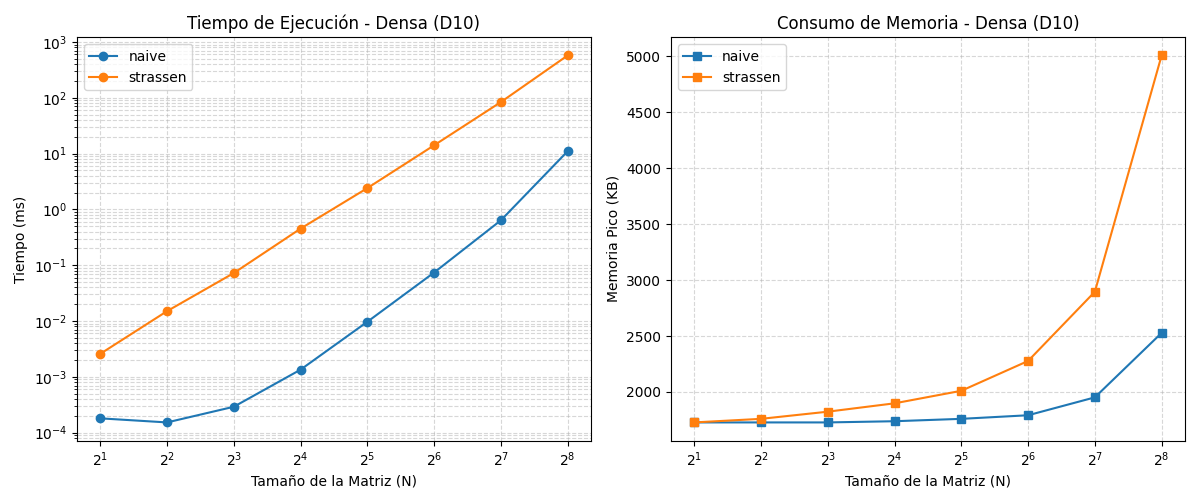
\includegraphics[width=\linewidth]{plots/matrix_densa_D10.png}
        \caption{Rendimiento en matrices densas ($D10$).}
        \label{fig:matrix_densa}
    \end{minipage}\hfill
    \begin{minipage}{0.48\textwidth}
        \centering
        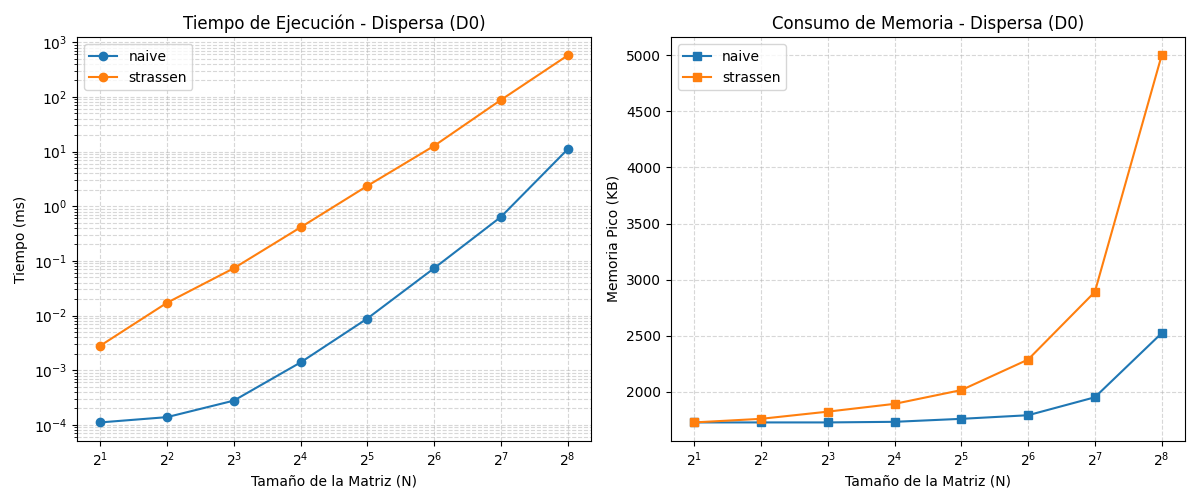
\includegraphics[width=\linewidth]{plots/matrix_dispersa_D0.png}
        \caption{Rendimiento en matrices dispersas ($D0$).}
        \label{fig:matrix_dispersa}
    \end{minipage}
\end{figure}

\begin{table}[htbp]
\centering
\small
\caption{Tiempo (ms) y memoria pico (KB) en multiplicación de matrices densas ($D10$).}
\label{tab:matrix_summary}
\begin{tabular}{rrrrr}
\toprule
& \multicolumn{2}{c}{\textbf{Tiempo de CPU (ms)}} & \multicolumn{2}{c}{\textbf{Memoria RAM Pico (KB)}} \\

\textbf{Dimensión ($N$)} & \textbf{Naive} & \textbf{Strassen} & \textbf{Naive} & \textbf{Strassen} \\
\midrule
$2^1 = 2$    & 0.0002 & 0.0026 & 1728 & 1728 \\
$2^4 = 16$   & 0.0013 & 0.4532 & 1739 & 1899 \\
$2^6 = 64$   & 0.0741 & 14.114 & 1792 & 2277 \\
$2^7 = 128$  & 0.6390 & 84.039 & 1952 & 2896 \\
$2^8 = 256$  & 11.064 & 575.37 & 2528 & 5008 \\
\bottomrule
\end{tabular}
\end{table}

\paragraph{Análisis de Desempeño y Sobrecarga Práctica:}
A pesar de que el Teorema Maestro establece para Strassen una cota asintótica estrictamente superior de $\mathcal{O}(N^{\log_2 7}) \approx \mathcal{O}(N^{2.81})$ frente a $\Theta(N^3)$ del método iterativo tradicional, los resultados experimentales demuestran que \textbf{el algoritmo Naive supera categóricamente a Strassen en todo el rango evaluado ($N \le 256$)}.

Esta aparente contradicción entre teoría y práctica se justifica mediante tres fenómenos del modelo computacional real:
\begin{enumerate}
    \item \textbf{Constante Oculta Desproporcionada:} En cada nivel del árbol de recursión, Strassen efectúa 18 sumas y restas de bloques de matrices de tamaño $(N/2) \times (N/2)$, además de alocar dinámicamente espacio para 21 matrices intermedias ($a, \dots, h$, $p_1, \dots, p_7$, auxiliares). La constante multiplicativa oculta en el término $\Theta(N^2)$ de la recurrencia $T(N) = 7T(N/2) + \Theta(N^2)$ es órdenes de magnitud mayor que la del bucle triple de Naive.
    \item \textbf{Dispersión de Memoria y Líneas de Caché:} Los tres bucles anidados de Naive acceden a posiciones secuenciales de memoria, aprovechando de forma óptima el principio de localidad espacial de las líneas de caché L1/L2. Strassen, al fragmentar los arreglos en matrices no contiguas en el \textit{heap}, multiplica los fallos de caché de datos (\textit{cache misses}).
    \item \textbf{Ausencia de Caso Base Híbrido:} El algoritmo de Strassen evaluado recurre de forma pura hasta submatrices de $1 \times 1$. En la literatura especializada se demuestra que para que Strassen sea competitivo, debe conmutar a multiplicación Naive cuando $N \le 64$ o $N \le 128$, y su punto de cruce real sobrepasa típicamente $N = 1024$ o $N = 2048$.
\end{enumerate}

\paragraph{Invarianza frente a la Dispersión:}
Se observa que las curvas para matrices densas, diagonales y dispersas son indistinguibles entre sí. Esto se debe a que ninguno de los dos algoritmos posee bifurcaciones condicionales que detecten coeficientes nulos; ambos aplican ciegamente la misma cantidad fija de operaciones aritméticas en el modelo \textit{word-RAM}.

\paragraph{Consumo de Memoria Residente:}
Tal como ilustra la Figura~\ref{fig:matrix_densa}, el consumo de memoria de Naive crece a una tasa cuadrática moderada asociada únicamente a las entradas $M_1, M_2$ y la salida $C$ ($\approx 2.5$ MB en $N=256$). Por su parte, Strassen escala de forma abrupta a partir de $N = 128$, alcanzando $\approx 5$ MB en $N=256$, producto de los múltiples marcos de pila y la retención de las matrices temporales $P_i$ en los diferentes niveles de la recursión.

\section{Conclusiones}
Los resultados experimentales ratifican que el comportamiento observable en arquitecturas físicas contemporáneas está fuertemente modulado por las constantes ocultas y la interacción con la jerarquía de memoria caché, más allá de la cota asintótica formal. En ordenamiento, los cuatro algoritmos verificaron la tasa $\mathcal{O}(n \log n)$, destacando la superioridad de \texttt{std::sort} (159.6 ms para $N = 10^7$ en aleatorio $D7$) debida a su baja sobrecarga interna frente al elevado costo espacial de PatienceSort ($\approx 184.6$ MB) originado por su gestión dinámica de pilas. Por su parte, en multiplicación matricial, a pesar de que Strassen ostenta una cota asintótica superior de $\mathcal{O}(n^{2.81})$ frente a $\Theta(n^3)$, el método Naive resultó más de 50 veces más rápido en $N = 256$ (11.06 ms vs. 575.37 ms), demostrando que la penalización por fallos de caché y las 18 adiciones/asignaciones de submatrices por nivel recursivo imposibilitan alcanzar el punto de cruce práctico en instancias pequeñas y medianas sin un esquema híbrido de corte.

\section{Implementaciones}
El código fuente completo de la tarea, incluyendo las implementaciones en C++17 de los algoritmos de ordenamiento y multiplicación matricial, los programas principales de medición, los generadores de instancias y los scripts de visualización, se encuentra disponible en el siguiente repositorio público de GitHub:

\begin{center}
    \url{https://github.com/cstobalduc/INF221-Tarea1} % Reemplaza con el enlace real de tu repositorio
\end{center}


\newpage
\begin{thebibliography}{9}

\bibitem{taocv3}
Donald E. Knuth.
\newblock \emph{The Art of Computer Programming, Volume 3: Sorting and Searching}.
\newblock Addison Wesley Longman Publishing Co., Inc., 2da edición, 1998.

\bibitem{algorithms_erickson}
Jeff Erickson.
\newblock \emph{Algorithms}.
\newblock 2019. ISBN: 978-1-792-64483-2.

\bibitem{geeksforgeeks}
GeeksforGeeks.
\newblock \emph{Sorting Algorithms and Matrix Multiplication Implementations}.
\newblock \url{https://www.geeksforgeeks.org/}, 2026.

\bibitem{cormen2009introduction}
Thomas H. Cormen, Charles E. Leiserson, Ronald L. Rivest y Clifford Stein.
\newblock \emph{Introduction to Algorithms}.
\newblock The MIT Press, 3ra edición, 2009.
\end{thebibliography}

\end{document}